\chapter{The Large Hadron Collider (LHC)}\label{chapter:LHC}

The Large Hadron Collider (\Gls{LHC}) at CERN is the world's most powerful superconducting hadron accelerator and collider that sits in the $26.7~\mathrm{km}$ tunnel originally housing CERN's Large Electron Position Collider (LEP) passing roughly $100~\mathrm{m}$ beneath the the borders of Switzerland and France.
The LHC tunnels form an octagon with rounded corners consisting of eight arcs and eight straight sections that connect eight \gls{interaction point}s (IP) where the beam paths can be brought to cross for collisions.
Four of those collision points are located at caverns that contain the main four experiments of the LHC: ATLAS~\cite{PERF-2007-01} at Point 1, CMS~\cite{CMS:2008} at Point 5, LHCb~\cite{LHCb:2008} at Point 8, and ALICE~\cite{ALICE:2008} at Point 2.
The other four interaction points are left intentionally unused for collisions and beam crossings are forgone to prevent unnecessary disruption of the beams~\cite{Evans:2008}.

\section{Design}

The LHC was designed to collide beams of protons at high energy with very high luminosity, with a design center of mass energy of $14~\TeV{}$ and a design maximum instantaneous luminosity\footnote{In the more familiar units of barns used by particle physicists, $10^{34}~\mathrm{cm}^{-2}\mathrm{s}^{-1}=10~\mathrm{nb}^{-1}\mathrm{s}^{-1}=0.036~\mathrm{fb}^{-1}\mathrm{hr}^{-1}$.} of $10^{34}~\mathrm{cm}^{-2}\mathrm{s}^{-1}$~\cite{Bruning:782076,Evans:2008}.
Given the extreme beam intensity required to reach such luminosities proton-anti-proton collisions (as was used successfully at Fermilab's Tevatron) are not feasible.
Instead, two counter circulating beams of protons are used which imposes the requirement of opposite magnetic dipole fields in the rings.\\

The proton beams are guided along the LHC by a complex system of superconducting magnets.
The system consists of 1,232 $8.3~\mathrm{T}$ dipole magnets responsible for bending the beam and 392 $7.5~\mathrm{T}$ main quadrupole magnets dedicated to focusing the beam and are complemented by many insertion quadrupole magnets to help suppress beam dispersion~\cite{Rossi:2003,Rossi:2004}.
The high magnetic fields require huge currents, with the main dipole magnets designed for a nominal current of $11,600~\mathrm{A}$.
To deliver this high of current while also staying superconducting the magnets are submerged in a liquid helium bath at $1.9~\mathrm{K}$ in a vacuum sealed inner vessel, as seen in \Cref{fig:LHC_dipole_cross_section}.
The magnetic coils that carry this current are assembled at CERN from copper stabilized NbTi Rutherford cables, as shown for similar cables in~\cite{CERN-FOOTAGE-2016-014-001}.

\begin{figure}[htbp]
 \centering
 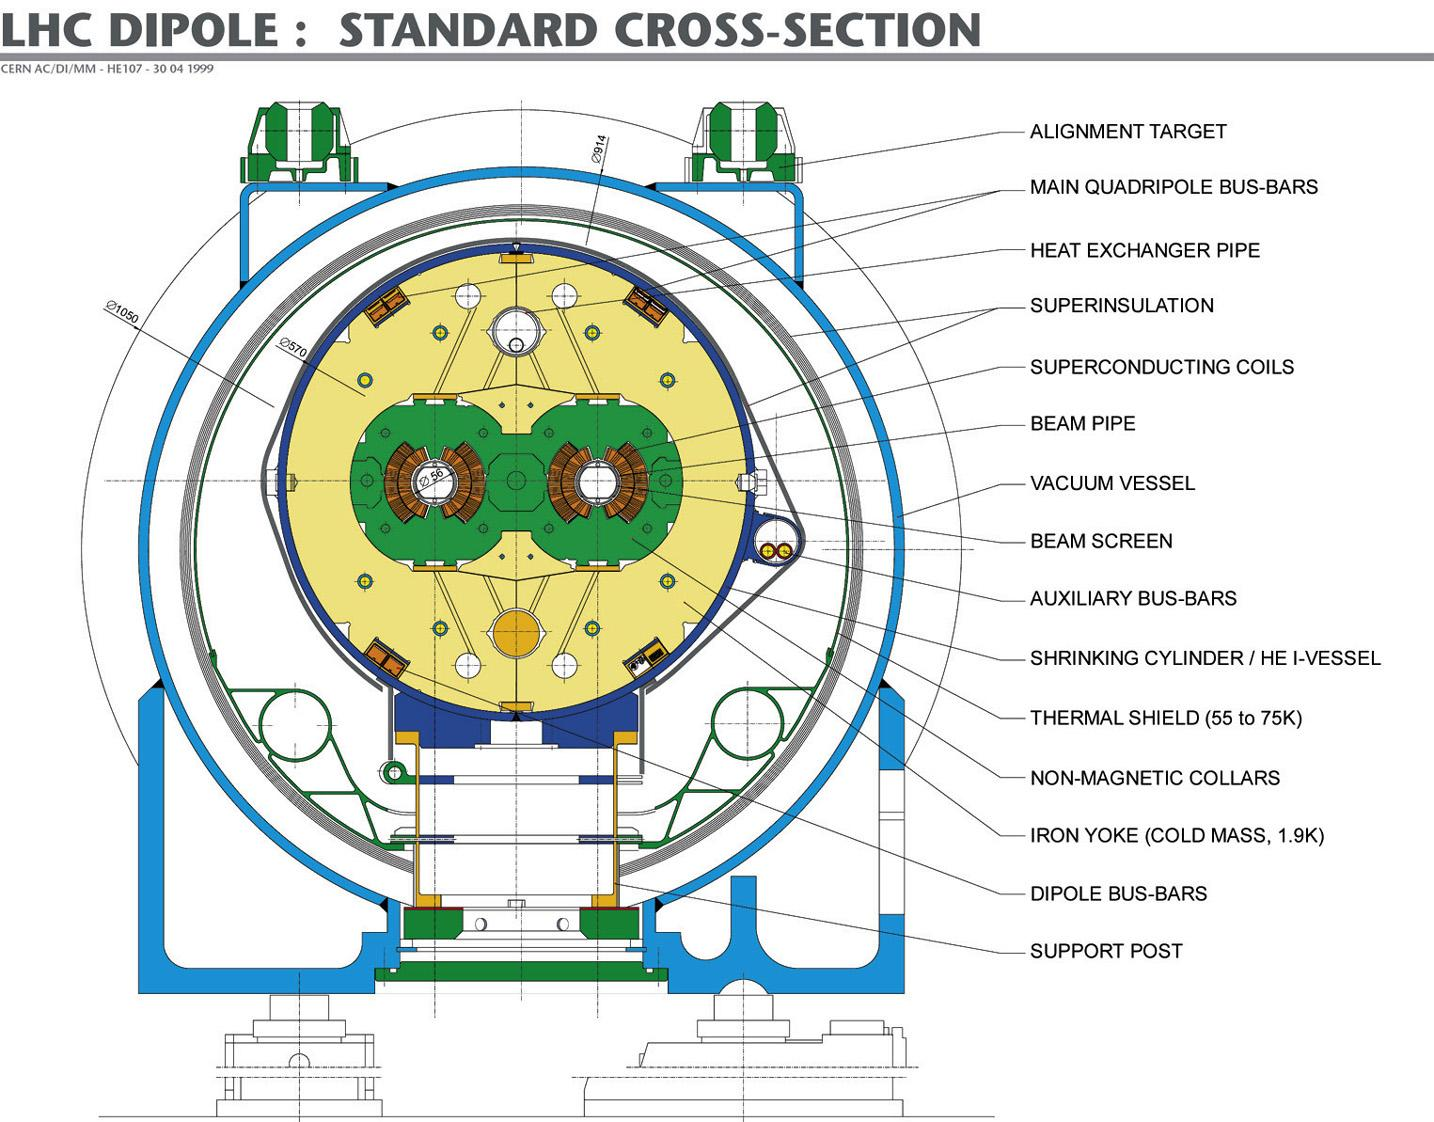
\includegraphics[width=0.6\textwidth]{LHC/LHC_dipole_cross_section.jpg}
 \caption{The cross-section of an LHC dipole magnet with cold mass and vacuum chamber~\cite{LHC:dipole}.}\label{fig:LHC_dipole_cross_section}
\end{figure}

\section{Accelerator}

The LHC is the last step for protons in a sequence of accelerators, as shown in \Cref{fig:LHC_accelerator_complex}, that increase the energy of the beams.
The protons start from a single bottle of Hydrogen gas\footnote{This is the same bottle that has been used since the very start of LHC operations, and given that the LHC can be refilled hundreds of thousands of times from one $\textrm{ml}$ of Hydrogen, a typical industrial bottle of Hydrogen will last for over a billion years of LHC operations.} at the site for the Linac2 linear accelerator.
The Hydrogen gas passes through an area of very high electrical field which ionizes the gas allowing for the electrons to be diverted away and for the protons to continue on.
The protons then enter Linac2, the first accelerator of the LHC injector chain, where they are accelerated to an energy of $50~\MeV$.
The proton beam is then split and injected into the four Proton Synchrotron Booster rings where the beams are accelerated to $1.4~\GeV$ before recombination and injection into the \Gls{Proton Synchrotron} (PS) where the beam is further accelerated to $25~\GeV$ and forms a bunch train with $25~\textrm{ns}$ spacing --- radio frequency (RF) harmonics with bunches of protons surfing the RF wave troughs.
In the penultimate stage of the injector chain, the beam is injected into the Super Proton Synchrotron where it reaches an energy of $450~\GeV$.
Finally, the protons are injected into the LHC and split into two countercirculating beams.
Once the beams are circulating in the LHC they are further accelerated while keeping the $25~\textrm{ns}$ spacing to their final energy of $6.5~\TeV$ by RF accelerator systems at Point 4~\cite{Evans:2008,Boussard:410377}.
The beams can circulate stably in the LHC for many hours and so only need to be refilled if the beam is dumped.

\begin{figure}[htbp]
 \centering
 \includegraphics[width=\textwidth]{LHC/LHC_accelerator_complex.jpg}
 \caption{Sketch of the CERN accelerator complex.
  The LHC (dark grey ring) is the last ring in a complex chain of particle accelerators, where smaller machines are used in a chain to help boost particles to their final energies and provide beams to a whole set of smaller experiments~\cite{Haffner:1621894}.
  The LHC proton injector chain is the indicated by the paths marked with light grey arrows.}\label{fig:LHC_accelerator_complex}
\end{figure}

\section{Collider}

The circulating proton beams in the LHC cross paths at the four interaction points where the main LHC experiments are located.
The collisions of the proton beams in the experiments have a resulting center of mass energy of $\sqrt{s} = 13~\TeV$ and, as shown by \Cref{eq:events_from_luminosity}, the number of events generated per second for a particular process is governed by the machine (instantaneous) luminosity, $\luminosity$, which for a beam shape that is Gaussianly distributed is
\begin{equation}
 \luminosity = \frac{N_{b}^{2} n_{b} f_{\mathrm{rev}} \,\gamma_{r}}{4 \pi \epsilon_{n} \beta^{*}} F
 \label{eq:machine_luminosity}
\end{equation}
where $N_{b}$ is the number of particles per bunch, $n_{b}$ is the number of bunches per beam, $f_{\mathrm{rev}}$ is the revolution frequency, $\gamma_{r}$ is the relativistic gamma factor, $\epsilon_{n}$ is the normalized transverse beam emittance, $\beta^{*}$ is the beta function at the collision point, and $F$ is the geometric luminosity reduction factor due to the crossing angle at the interaction point:
\[
 F = \left(1 + \left(\frac{\theta_{c} \,\sigma_{z}}{2 \sigma^{*}}\right)\right)^{-1/2},
\]
where $\theta_{c}$ is the full crossing angle at the interaction point, $\sigma_{z}$ is the RMS bunch length, and $\sigma^{*}$ is the transverse RMS beam size at the interaction point~\cite{Evans:2008}.
Nominal design values for these quantities are given in \Cref{table:LHC_collider_parameters}, which additionally shows the incredibly successfully results of the LHC operations and accelerator teams' operation of the LHC in Run II.
From \Cref{eq:events_from_luminosity} and \Cref{eq:machine_luminosity} it is seen that to obtain the high number of hard collisions to have sensitivity to new physics both high beam energies and high luminosities are required.
As can be seen from \Cref{eq:machine_luminosity}, one approach to increasing the luminosity in the future for the High-Luminosity LHC (HL-LHC) is to decrease $\beta^{*}$ through the use of more powerful quadrupole focusing magnets.
However, this requires a larger crossing angle, decreasing the geometric factor, but this can be compensated for by the use of crab cavities~\cite{PhysRevAccelBeams.19.101003}.

\begin{table}[htpb]
 \centering
 \caption{Nominal design values of LHC operations parameters at ATLAS for $25~\textrm{ns}$ bunch crossing spacing~\cite{Evans:2008,PhysRevAccelBeams.19.101003}.
  Design and ATLAS recorded values of the machine luminosity are also given for LHC Run II operations~\cite{TWiki:2018ATLASPeakLumi}.
 }
 \begin{tabular}{@{}llr@{}} \toprule
  Parameter                                   & Symbol             & LHC Run II Value                     \\ \midrule
  LHC circumference                           &                    & $26,659~\mathrm{m}$                  \\
  LHC beam energy                             &                    & $7~\TeV$                             \\
  LHC beam energy in Run II                   &                    & $6.5~\TeV$                           \\
  Number of protons per bunch                 & $N_{b}$            & $1.15 \times 10^{11}$                \\
  Number of proton bunches per beam           & $n_{b}$            & $2,808$                              \\
  Revolution frequency                        & $f_{\textrm{rev}}$ & $11.245~\mathrm{kHz}$                \\
  Lorentz factor                              & $\gamma_{r}$       & $7462.69$                            \\
  Lorentz factor at $\sqrt{s} = 13~\TeV$      &                    & $6929.64$                            \\
  Normalized transverse beam emittance        & $\epsilon_{n}$     & $3.75~\mu\mathrm{m}$                 \\
  Collision point beta function               & $\beta^{*}$        & $0.55~\mathrm{m}$                    \\
  Full crossing angle                         & $\theta_{c}$       & $285~\mu\mathrm{rad}$                \\
  RMS bunch length                            & $\sigma_{z}$       & $7.55\times 10^{-2}~\mathrm{m}$      \\
  Transverse RMS beam size                    & $\sigma^{*}$       & $16.6~\mu\mathrm{m}$                 \\ \midrule
  Peak design machine luminosity at $14~\TeV$ & $\luminosity$      & $10~\mathrm{nb}^{-1}\mathrm{s}^{-1}$ \\
  Peak design machine luminosity at $13~\TeV$ &                    & $9~\mathrm{nb}^{-1}\mathrm{s}^{-1}$  \\
  Peak ATLAS recorded machine luminosity      &                    & $21~\mathrm{nb}^{-1}\mathrm{s}^{-1}$ \\
  \bottomrule
 \end{tabular}\label{table:LHC_collider_parameters}%
\end{table}
